\section{Hyper-parameters}
\subsection{Reward Functions}
\label{app:rewards}
The reward functions we used during the training are shown in Table~\ref{reward}, which come from \cite{kumar2021rma, agarwal2023legged, margolis2023walk, fu2021minimizing}.

\begin{table}[h]
    \centering
    \caption{Rewards}
    \begin{tabular}{lll}
    \toprule[1.5pt] Reward & Equation $\left(r_i\right)$ & Weight $\left(w_i\right)$ \\
    \midrule[1.5pt] Lin. velocity tracking & $\exp \left\{- \frac{\|\mathbf{v}_{x y}^{\text {cmd }}-\mathbf{v}_{x y}\|_2^2}{\sigma}  \right\}$ & 1.0 \\
    Ang. velocity tracking & $\exp \left\{- \frac{\left(\omega_{\text {yaw }}^{\text {cmd }}-\omega_{\text {yaw }}\right)^2}{\sigma} \right\}$ & 0.5 \\
    Linear velocity $(z)$ & $v_z^2$ & -2.0 \\
    Angular velocity $(x y)$ & $\|\boldsymbol{\omega}_{x y}\|_2^2$ & -0.05 \\
    Orientation & $\|\mathbf{g}\|_2^2$ & -0.2 \\
    Joint accelerations & $\|\ddot{\boldsymbol{\theta}}\|^2$ & $-2.5 \times 10^{-7}$ \\
    Joint power & $|\boldsymbol{\tau} \| \dot{\boldsymbol{\theta}}|^{T}$ & $-2 \times 10^{-5}$ \\
    Body height & $\left(h^{\text {target}}-h\right)^2$ & -1.0 \\
    Foot clearance & $\sum_{i=0}^{3}\left(p_{z}^{\text {target}}-p_{z}^{i}\right)^2 \cdot v_{xy}^{i}$ & -0.01 \\
    Action rate & $\|\mathbf{a}_t-\mathbf{a}_{t-1}\|_2^2$ & -0.01 \\
    Smoothness & $\|\mathbf{a}_t-2 \mathbf{a}_{t-1}+\mathbf{a}_{t-2}\|_2^2$ & -0.01 \\
    \bottomrule[1.5pt]
    \end{tabular}
    % \caption{Rewards}
    \label{reward}
\end{table}

In Table~\ref{reward}, $\sigma$ is the tracking shaping scale and we use $\sigma = 0.25$, $h^{\text{target}}$ is the desired base height corresponding to ground, $p_z^{\text{target}}$ and $p_z^i$ are the desired feet position and real feet position in z-axis of robot's frame and $v_{xy}^i$ is the feet velocity in xy-plane of robot's frame.

\subsection{Domain Randomizations}
\label{app:rand}
For the training of our method and other methods, domain randomizations we use are shown in Table~\ref{randomization}, which come from \cite{wu2023learning, nahrendra2023dreamwaq}.

\begin{table}[h]
    \centering
    \caption{Domain Randomizations and their Respective Range}
    \begin{tabular}{lll}
    \toprule[1.5pt] Parameters & Range[Min, Max] & Unit \\
    \midrule[1.5pt]
    Body Mass & {$[0.8,1.2] \times$ nominal value } & $\mathrm{Kg}$ \\
    Link Mass & {$[0.8,1.2] \times$ nominal value } & $\mathrm{Kg}$ \\
    CoM & {$[-0.1,0.1] \times [-0.1,0.1] \times [-0.1,0.1]$} & $\mathrm{m}$ \\
    Payload Mass & {$[-1,3]$} & $\mathrm{Kg}$ \\
    Ground Friction & {$[0.2,2.75]$} & - \\
    Ground Restitution & {$[0.0,1.0]$} & - \\
    Motor Strength & {$[0.8,1.2] \times$ motor torque } & $\mathrm{Nm}$ \\
    Joint $K_p$ & {$[0.8,1.2] \times 20$} & - \\
    Joint $K_d$ & {$[0.8,1.2] \times 0.5$} & - \\
    Initial Joint Positions & {$[0.5,1.5] \times$ nominal value } & $\mathrm{rad}$ \\
    System Delay & {$[0,3\Delta_t]$ } & $\mathrm{s}$ \\
    External Force & {$[-30, 30] \times [-30, 30] \times [-30, 30]$} & $\mathrm{N}$ \\
    \bottomrule[1.5pt]
    \end{tabular}
    % \caption{dynamics Randomization and Their Respective Range}
    \label{randomization}
\end{table}

\newpage
\subsection{Training Terrains}
\label{app:terrain}

Our terrain comprises slopes, rough slopes, stairs, and discrete obstacles. 

The slopes and rough slopes vary in inclination from 0$^{\circ}$ to 40$^{\circ}$ with the addition of uniform noise ranging from $\pm$ 1 cm to $\pm$ 8 cm on the rough slopes. The stairs have random widths ranging from 20 cm to 40 cm and heights varying from 5 cm to 23 cm. The discrete obstacles have heights ranging from $\pm$ 5 cm to $\pm$ 15 cm. We assign difficulty levels to the terrains using integers from 0 to 9. More specifically, for a terrain level indicated by $\text{level}^{\text{terrain}}$, the corresponding terrains are as follows: \\

$\bullet$ Slopes: with inclination of $40 \times \frac{\text{level}^{\text{terrain}}}{9}$ $^{\circ}$; \\
$\bullet$ Rough slopes: with amplitude of $1 + 7 \times \frac{\text{level}^{\text{terrain}}}{9}$ cm and inclination of $40 \times \frac{\text{level}^{\text{terrain}}}{9}$ $^{\circ}$; \\
$\bullet$ Stairs: with step height of $5 + 18 \times \frac{\text{level}^{\text{terrain}}}{9}$ cm; \\
$\bullet$ Discrete obstacles: with height of $5 + 10 \times \frac{\text{level}^{\text{terrain}}}{9}$ cm.
The proportion of the above terrains is 0.1, 0.2, 0.6, and 0.1 correspondingly.

\subsection{Hyper Parameters}
\label{app:hyper}
\begin{table}[H]
\centering
\caption{Hyper Parameters for Training}
\begin{tabular}{@{}cc@{}}
\toprule[1.5pt]
General                          &              \\ \midrule[1.5pt]
Batch   Size                     & 4096 $\times$ 200 \\
Mini-batch   Size                & 4096 $\times$ 50  \\
Number   of epochs               & 5            \\ \midrule[1.5pt]
PPO                              &              \\ \midrule[1.5pt]
Clip   range                     & 0.2          \\
Entropy   coefficient            & 0.01         \\
Discount   factor                & 0.99         \\
GAE   discount factor            & 0.95         \\
Desired   KL-divergence          & 0.01         \\
Learning   rate                  & 1 $\times \, 10^{-3}$         \\
Adam   epsilon                   & 1 $\times \, 10^{-8}$         \\
Gradient   clipping              & 10           \\ \midrule[1.5pt]
HIM                              &              \\ \midrule[1.5pt]
Number   of prototypes           & 16           \\
Contrastive   loss scale         & 1.0          \\
Velocity   estimation loss scale & 1.0          \\
Learning   rate                  & 1 $\times \, 10^{-3}$         \\
Adam   epsilon                   & 1 $\times \, 10^{-8}$         \\
Gradient   clipping              & 10           \\ \bottomrule[1.5pt]
\end{tabular}
\end{table}


\newpage
\section{Experimental Details}

\subsection{Real-world Benchmark Setup}
\label{app:real}
Our benchmark consists of three parts: \textbf{stairs}, \textbf{unseen terrains} and \textbf{anti-disturbance}:

\paragraph{Stairs:} \\
$\bullet$ Short-range stairs: This scene includes two sets of stairs with 5 steps each. The height and width of the stairs are 16 cm and 27 cm, respectively. The Unitree A1 robot is used to test our policy in this scene, and the metric is the success rate of going through both stairs. The corresponding snapshots of this scene are displayed in the left column of Fig.~\ref{fig:stairs}. \\
$\bullet$ Long-range stairs: This scene consists of hundreds of stairs with a height of 17 cm and a width of 25 cm. The Unitree Aliengo robot is equipped with policies that need to be tested, and the metric is the number of stairs the robot can ascend without stopping. The corresponding photos of this scene are shown in the right column of Fig.~\ref{fig:stairs}. \\

\paragraph{Unseen terrains:} \\
$\bullet$ Compositional terrain: This scene alternates between gravel and stairs, as depicted in the upper picture of Fig.~\ref{fig:unseen}. The Unitree Aliengo robot is equipped with policies that need to be tested, and the metric is the success rate of going through three compositional alternations. \\
$\bullet$ Deformable slope: This scene makes a deformable slope created by two soft beds, as shown in the lower picture of Fig.~\ref{fig:unseen}. The Unitree A1 robot is used to test our policy, and the metric is the success rate of navigating through this slope. \\

\paragraph{Anti-disturbance:} \\
$\bullet$ Dragging obstacle: This task simulates the scenario where the robot's leg is dragged by obstacles. A wooden box is attached to the robot's back leg, preventing its movement. The metric for this task is the maximum weight the robot can handle. The Unitree A1 robot is used, and the illustration can be found in the top-left of Fig.~\ref{fig:disturbance}. \\
$\bullet$ Lateral hit: This task evaluates the robot's push-recovery ability. The robot is subjected to a lateral force from a load swinging down from a height of 107 cm. The Unitree A1 robot is used in this task, and the metric is the maximum weight of the load that the robot can withstand after being hit. The illustration is shown in the top-right of Fig.~\ref{fig:disturbance}. \\
$\bullet$ Payload: This task assesses the robot's carrying capacity. The Unitree A1 robot is used, and the maximum weight that the robot can carry while walking is measured. The illustration can be found in the bottom-left of Fig.~\ref{fig:disturbance}. \\
$\bullet$ Missing step: 
This task simulates the robot's reaction when it misses steps and falls from a high platform. The platform's height, as shown in the bottom-right of Fig.~\ref{fig:disturbance}, is 42 cm. The Unitree Aliengo robot is used in this task, and the metric is the success rate of maintaining balance after descending.

\begin{figure}[H]
    \centering
    \subfigure[Stairs]{
        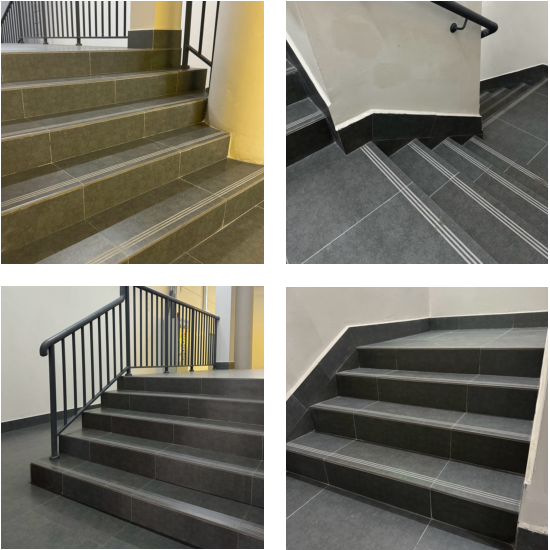
\includegraphics[width=0.313\textwidth]{exp-setup-1.pdf}
        \label{fig:stairs}
    }
    \subfigure[Unseen terrains]{
        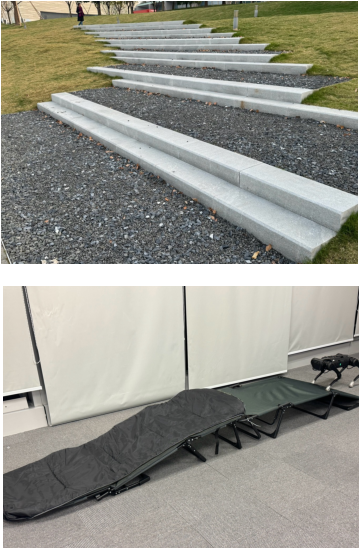
\includegraphics[width=0.205\textwidth]{exp-setup-2.pdf}
        \label{fig:unseen}
    }
    \subfigure[Anti-disturbance]{
    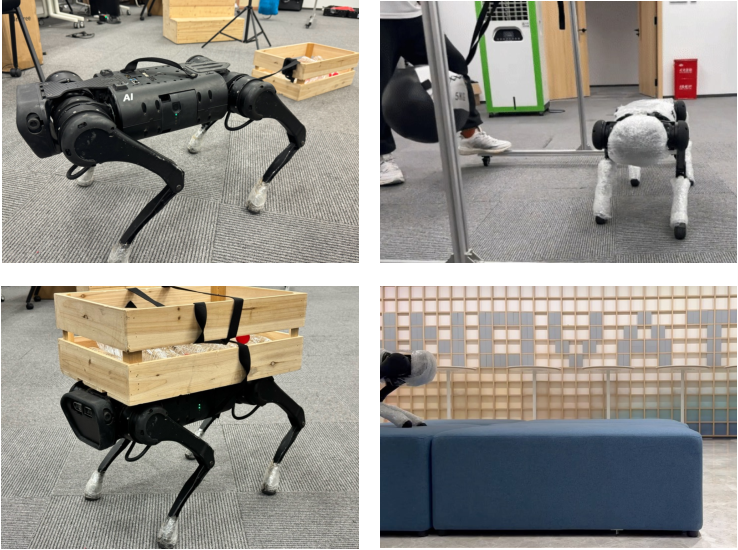
\includegraphics[width=0.42\textwidth]{exp-setup-3.pdf}
    \label{fig:disturbance}
    }
    \caption{Snapshots of our real-world scene benchmarks for quantitative analysis in Section~\ref{exp:real}.}
    \label{fig:benchmark}
\end{figure}

\subsection{Simulation Benchmark Setups}
\label{app:simu}

We consider tracking tasks with 3 different ranges of commands for each type of terrain. The tracking error on slopes and rough slopes are tested in the range $[-1.0,\, 1.0] \,\text{m/s} \times [-1.0,\, 1.0] \,\text{m/s} \times [-1.0,\, 1.0] \,\text{rad/s}$ and $[-2.0,\, 2.0] \,\text{m/s} \times [-1.0,\, 1.0] \,\text{m/s} \times [-2.0,\, 2.0] \,\text{rads/s}$. All other tests are conducted within the range $[-1.0,\, 1.0] \,\text{m/s} \times [-1.0,\, 1.0] \,\text{m/s} \times [-1.0,\, 1.0] \,\text{rad/s}$. These ranges correspond to linear velocity in the forward direction, lateral directions, and angular velocity about the vertical axis, respectively.

When testing the linear velocity tracking error, the angular velocity target is set to 0. For the angular velocity tracking error tests, the linear velocity target is 0. The 'combined velocity' tests are conducted without setting either velocity component to 0. We uniformly sample test commands within these ranges. The environmental conditions are set to $\text{level}^{\text{terrain}} = 1, 2, 3, 4$, with an equal distribution of 25\% for each, as explained in Appendix ~\ref{app:terrain}.


\subsection{Ablation on Number of prototypes}
\label{num_proto}

We conducted ablation studies on the number of prototypes in our research. By default, we set the number of prototypes to 16, which corresponds to the square of terrain types. 

The training curves for different numbers of prototypes are shown in Fig.~\ref{proto_score}. 
It can be observed that the performance of our method steadily improves as the number of prototypes increases until it reaches 64. After this, the performance starts to decline. 

This finding suggests that the representation of environmental dynamics does not require dense representation like pure regression, but overly sparse representation is also inadequate. 
Additionally, a high number of prototypes accelerates training during the initial stages but compromises final performance. Conversely, a low number of prototypes may lead to slower initial training but ultimately achieves superior final performance. 

Thus, determining an appropriate number of prototypes is vital for striking a balance between rapid training speed and optimal final performance. This matter warrants further investigation in future studies.

\begin{figure}[H]
    \centering
    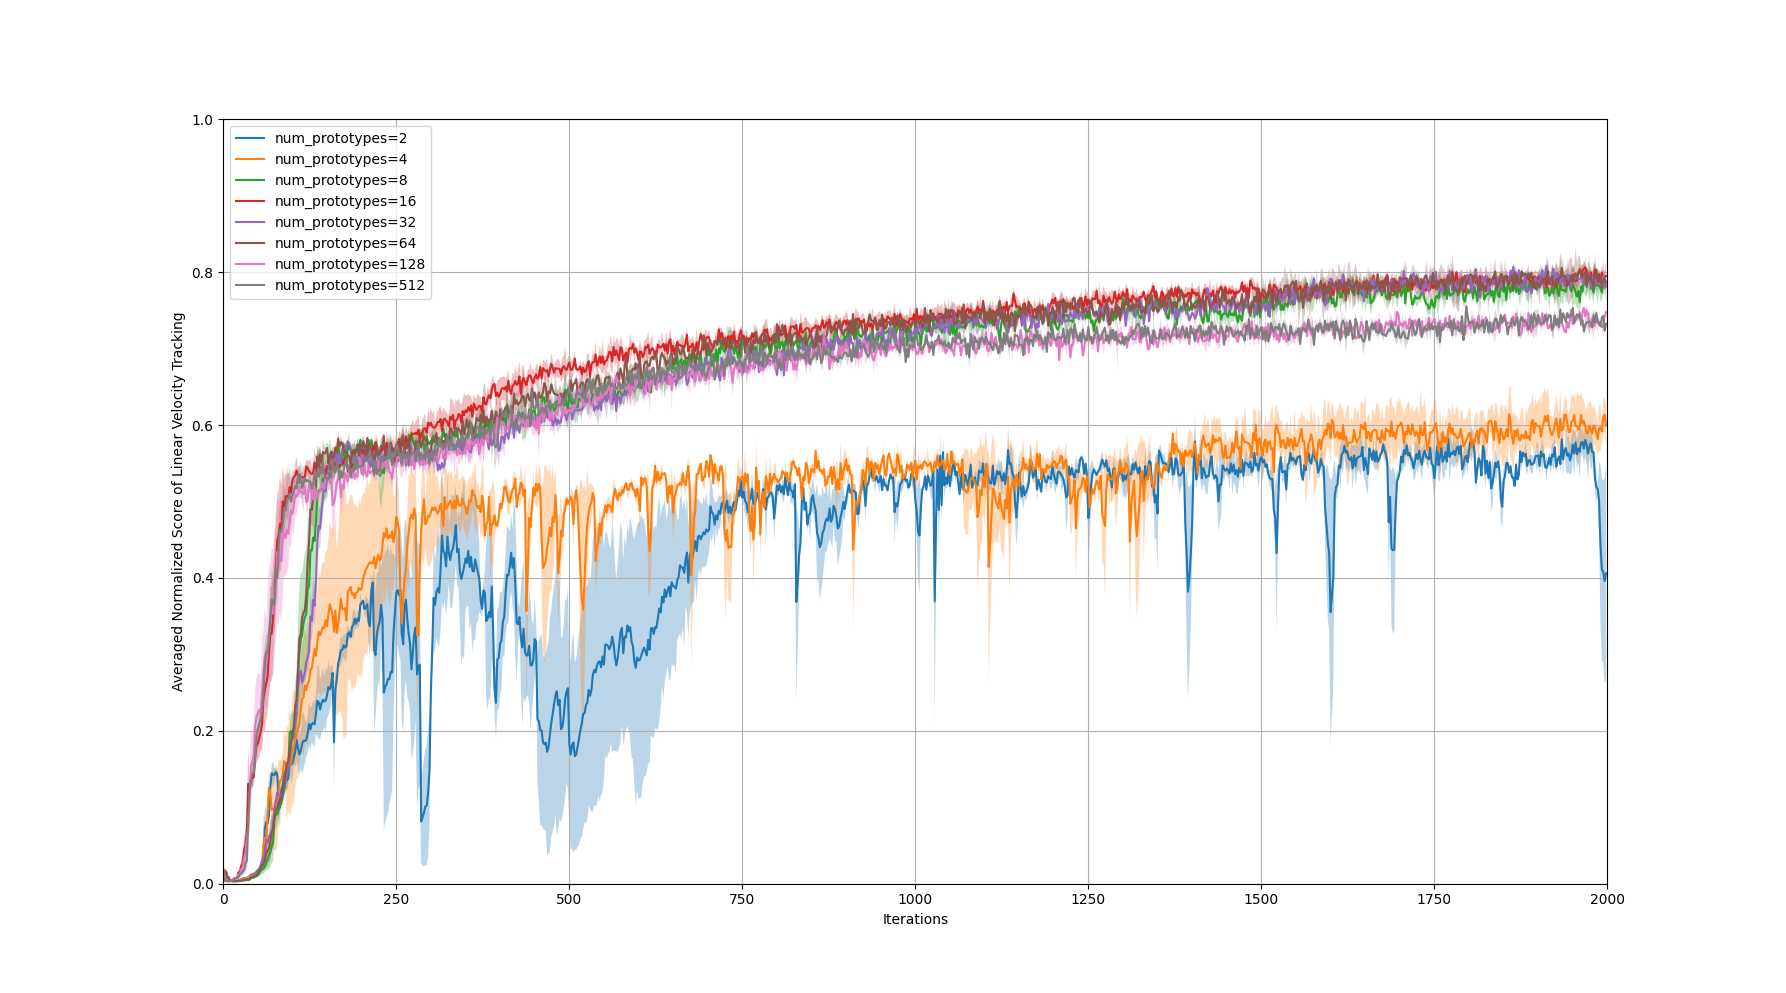
\includegraphics[width=1.0\textwidth]{proto_score.png}
    \caption{Normalized Linear Tracking Score over the number of Prototypes}
    \label{proto_score}
\end{figure}

\newpage
\subsection{Outdoor experiments}
We further evaluated our policy in additional real-world scenes. Videos can be found at the following \href{https://junfeng-long.github.io/HIMLoco/}{URL}. Illustrations of the scenes that have appeared during our outdoor experiments are shown in Fig.~\ref{fig:outdoor}.

\begin{figure}[H]
    \centering
    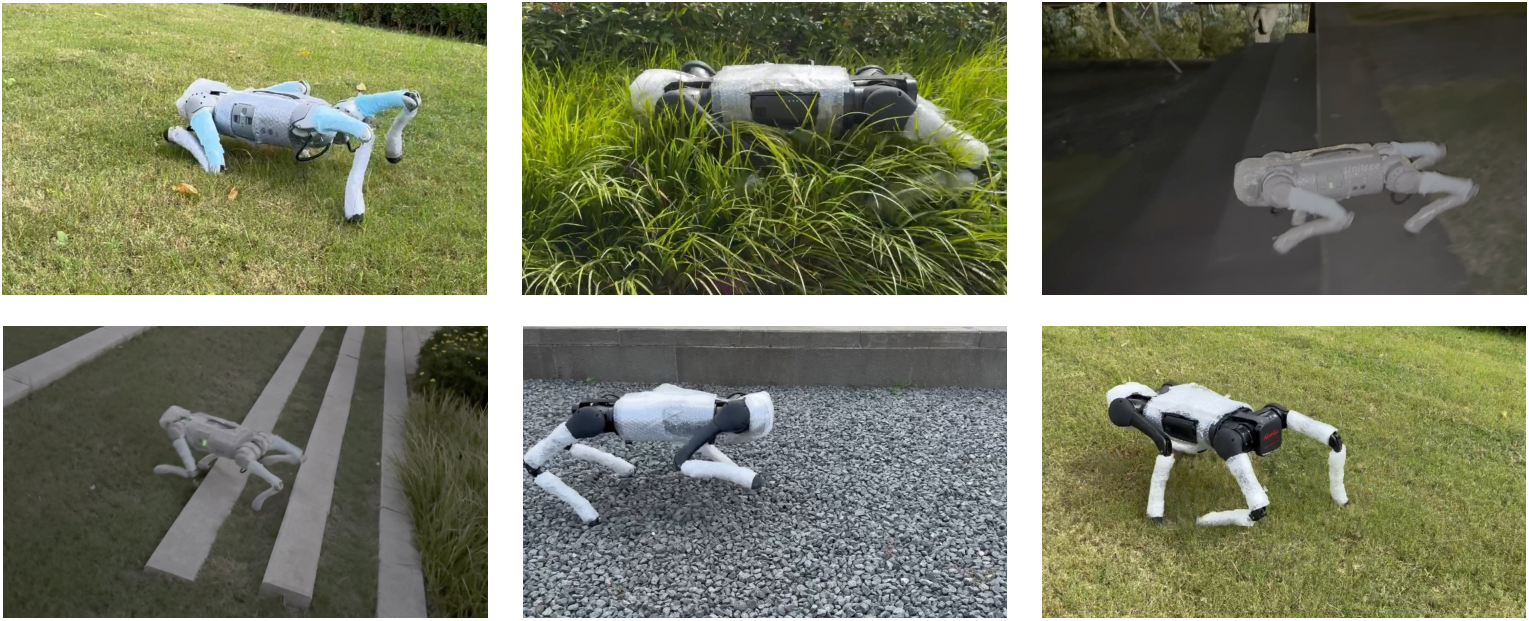
\includegraphics[width=1.0\textwidth]{outdoor_scene.pdf}
    \caption{Snapshots of various outdoor scenes for the agility evaluation of our quadruped robot.}
    \label{fig:outdoor}
\end{figure}
